\section{所提方法}
\label{sec:propo_approch}

沿用文献~\cite{deyPassivityBasedDecentralizedCriteria2023,chenExtendedFrequencyDomainPassivity2025a} 的思路，我们指出扇形性并不是系统的固有属性，而取决于输入和输出的具体选择。因此，改用其他变量可能使系统呈现扇形性。

\subsection{功率--极坐标系}
对于 GFM 变流器，一种特别合适的选择是采用功率--极坐标表示：以电压幅值和相位为输入，以有功和无功功率为输出。文献~\cite{deyAnalysisPassivityCharacteristics2021} 表明，这种表示在低频范围内给出 GFM 变流器的无源映射，因此系统具有扇形性。对每台变流器 $i$，相应的线性化变量变换由式~\eqref{eq:change_of_coord_1}--\eqref{eq:change_of_coord_2} 给出，其中变换矩阵 $\mathcal{E}_i$、$\mathcal{F}_i$ 和 $\mathcal{C}_i$ 取决于电压与电流运行点。
\begin{equation}
\begin{bmatrix}
\phi_i\\ |V|_i
\end{bmatrix}
=
\underbrace{
\begin{bmatrix}
-V^i_{q,0} & \dfrac{V^i_{d,0}}{\sqrt{(V^i_{d,0})^2+(V^i_{q,0})^2}}\\
V^i_{q,0} & \dfrac{V^i_{q,0}}{\sqrt{(V^i_{d,0})^2+(V^i_{q,0})^2}}
\end{bmatrix}}_{:=\mathcal{F}_i^{-1}}
\begin{bmatrix}V_{D,i}\\V_{Q,i}\end{bmatrix}.
\label{eq:change_of_coord_1}
\end{equation}

\begin{equation}
\begin{bmatrix}P_i\\Q_i\end{bmatrix}
=\underbrace{\begin{bmatrix}
V^i_{d,0}&V^i_{q,0}\\
V^i_{q,0}&-V^i_{d,0}
\end{bmatrix}}_{:=\mathcal{E}_i}
\begin{bmatrix}I_{D,i}\\I_{Q,i}\end{bmatrix}
+\underbrace{\begin{bmatrix}
I^i_{d,0}&V^i_{q,0}\\
-I^i_{q,0}&I^i_{d,0}
\end{bmatrix}}_{:=\mathcal{C}_i}
\begin{bmatrix}V_{D,i}\\V_{Q,i}\end{bmatrix}.
\label{eq:change_of_coord_2}
\end{equation}

据此，变流器的新输入--输出关系为式~\eqref{eq:pp_trasnf}；网络采用类似变换，得到式~\eqref{eq:pp_trasnf_net}：
\begin{equation}
J_{C,i}(s):=(\mathcal{E}_iY_{C_i}(s)+\mathcal{C}_i)\mathcal{F}_i,
\label{eq:pp_trasnf}
\end{equation}
\begin{equation}
\mathbf{J}_{net}(s):=(\boldsymbol{\mathcal{E}}\mathbf{Y}_{net}(s)-\boldsymbol{\mathcal{C}})\boldsymbol{\mathcal{F}}.
\label{eq:pp_trasnf_net}
\end{equation}
$\boldsymbol{\mathcal{E}}$、$\boldsymbol{\mathcal{C}}$ 和 $\boldsymbol{\mathcal{F}}$ 分别由 $\mathcal{E}_i$、$\mathcal{C}_i$ 和 $\mathcal{F}_i$ 构成块对角矩阵。$\mathcal{C}$ 前的负号源于网络电流方向与变流器中采用的电流方向相反。类似式~\eqref{eq:block_diagonal}，用 $\mathbf{J}_C$ 表示由 $J_{C_i}$ 构成的块对角矩阵。

如图~\ref{fig:loop_shaping} 所示，这一变量变换可以解释为环路变换。假设变换定义良好，则变换前后的输入--输出稳定性等价。系统稳定性由 $\det(\mathbf{Y}_{net}(s)+\mathbf{Y}_C(s))$ 的零点决定；由于
$\det(\mathbf{J}_C(s)+\mathbf{J}_{net}(s))=\det(\boldsymbol{\mathcal{E}}(\mathbf{Y}_{net}(s)+\mathbf{Y}_C(s))\boldsymbol{\mathcal{F}})$，变换前后系统的零点相同。此外，若不存在右半平面极零相消，则输入--输出稳定性蕴含内部稳定性，例如文献~\cite{häberle2025decentralizedparametricstabilitycertificates} 所示。因此，可以无损一般性地将定理~\ref{thm:dec_mixed_small_gain_phase} 直接用于变换后的系统。

\begin{figure}
\centering
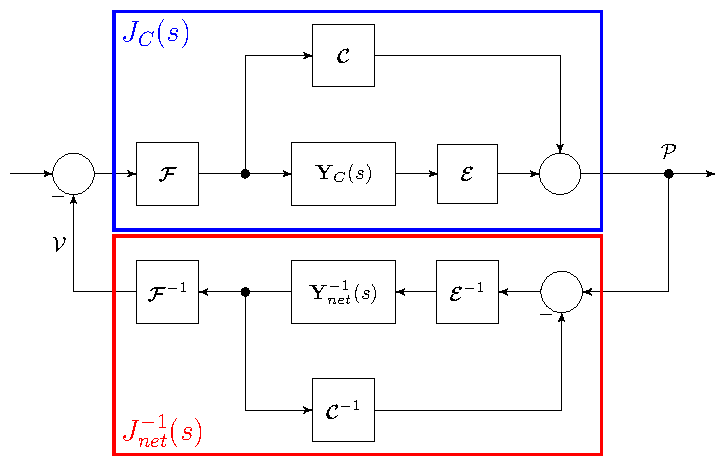
\includegraphics[width=\linewidth]{loop_shaping.pdf}
\caption{将所提变换解释为环路整形变换。}
\label{fig:loop_shaping}
\end{figure}

\begin{rem}
所提变换结合了文献~\cite{woolcockMixedGainPhase2023,chenExtendedFrequencyDomainPassivity2025a,deyPassivityBasedDecentralizedCriteria2023} 中的右乘与整形函数。式~\eqref{eq:pp_trasnf} 同时采用左乘、右乘以及平移项 $\mathcal{C}$。
\end{rem}

对式~\eqref{eq:frame_embedding} 的 GFM 模型应用该变换，直接计算可知 $J_C(s)$ 在零频率处等于式~\eqref{eq:J_C_0}，其中 $\gamma$ 为某个标量。在这种表示中，相位突变不会引起任何稳态功率偏差，电压幅值偏差只会导致无功功率变化。该矩阵为对角矩阵，特征值为 $0$ 和 $\gamma$，数值域是连接这两个特征值的线段。
\begin{equation}
J_C(0)=\begin{bmatrix}0&0\\0&\gamma\end{bmatrix}.
\label{eq:J_C_0}
\end{equation}

在此坐标系中，变流器零频导纳是相位定义良好的拟扇形矩阵。尽管这一性质未必延伸到整个低频段，但它仍是一个积极信号。要应用小相位判据，$\mathbf{J}_C(s)$ 和 $\mathbf{J}_{net}^{-1}(s)$ 必须在整个频率范围内都满足扇形性。该变换可以解决低频非扇形性，却不能保证高频段继续保持扇形性。

为说明这一点，再次分析接入无限大母线的同一台 GFM 变流器。小相位判据结果如图~\ref{fig:pp_frame_cond} 所示。变流器在约 $64$ Hz 以下具有扇形性，并且在这一范围内满足小相位条件。超过该频率后，变流器和网络都不再具有扇形性，判据因而失效。这说明该变换虽然解决了占主导地位的低频限制，却未完全消除小相位方法的适用性限制。

\begin{rem}
尽管 $\mathbf{J}_C(s)$ 继承了 $\mathbf{Y}_C(s)$ 的稳定性，但 $\mathbf{J}_{net}^{-1}(s)$ 未必如此。网络侧变换可解释为反馈运算，因而可能使系统失稳。因此，在应用定理~\ref{thm:dec_mixed_small_gain_phase} 之前，必须验证 $\mathbf{J}_{net}^{-1}(s)$ 的稳定性。
\end{rem}

\begin{figure}
\centering
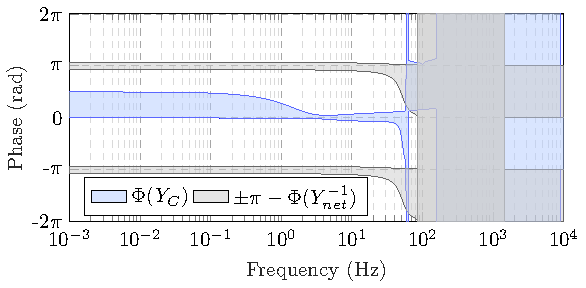
\includegraphics[width=\linewidth]{Phase_polar.pdf}
\caption{功率--极坐标系下 GFM 变流器的小相位条件。}
\label{fig:pp_frame_cond}
\end{figure}

\subsection{统一方法}
如上一节所示，无论采用标准直角坐标导纳系还是功率--极坐标系，相应判据都不能覆盖整个频率范围。在直角坐标系中，高频段（例如 $f>0.7$ Hz）相位定义良好且满足小相位条件；而对于极坐标系下经过环路整形的系统，低频段（例如 $f<64$ Hz）相位定义良好并满足小相位条件。

一种直观做法是组合两种坐标系：高频采用直角坐标系的相位，低频采用极坐标系的相位，只要每个频率上至少有一个坐标系满足小相位判据，就宣布系统稳定。然而，可以构造反例说明，不能简单合并不同坐标系的逐频率结果来推断稳定性。根本原因在于不同变换所界定的量不同：当 $\mathcal{C}$ 不是零矩阵时，$\mathbf{J}_C(j\omega)\mathbf{J}_{net}^{-1}(j\omega)$ 与 $\mathbf{Y}_C(j\omega)\mathbf{Y}_{net}^{-1}(j\omega)$ 的特征值通常并不相同。

为将两种坐标系统一到同一个系统中，令整形矩阵 $\mathcal{E}_i$、$\mathcal{F}_i$ 和 $\mathcal{C}_i$ 成为频率相关矩阵：
\begin{equation}
\begin{aligned}
\tilde{J}_{C_i}(s)&=(\mathcal{E}_i(s)Y_{C_i}(s)+\mathcal{C}_i(s))\mathcal{F}_i(s),\\
\tilde{\mathbf{J}}_{net}(s)&=(\boldsymbol{\mathcal{E}}(s)\mathbf{Y}_{net}(s)-\boldsymbol{\mathcal{C}}(s))\boldsymbol{\mathcal{F}}(s).
\end{aligned}
\label{eq:generic_trasnf}
\end{equation}
这些矩阵的选择必须保证每个 $\tilde{J}_{C_i}(s)$ 以及 $\tilde{\mathbf{J}}_{net}^{-1}(s)$ 均稳定。此外，若 $\boldsymbol{\mathcal{E}}(s)$、$\boldsymbol{\mathcal{C}}(s)$ 和 $\boldsymbol{\mathcal{F}}(s)$ 构成的整形变换适定，则由 $\tilde{\mathbf{J}}_C$ 与 $\tilde{\mathbf{J}}_{net}$ 构成的环路整形系统和由 $\mathbf{Y}_C$ 与 $\mathbf{Y}_{net}$ 构成的原系统具有相同的稳定性。这种表述在选择变换矩阵时十分灵活，但要找到能够同时保证开环稳定性和全频段扇形性的矩阵并不容易。

理想情况下，低频矩阵应与式~\eqref{eq:change_of_coord_1}--\eqref{eq:change_of_coord_2} 中的矩阵一致，以下记为 $\mathcal{E}_{J,i}$、$\mathcal{F}_{J,i}$ 和 $\mathcal{C}_{J,i}$；高频矩阵则应回到直角坐标系，即 $\mathcal{E}=\mathcal{F}=I$、$\mathcal{C}=0$，以下记为 $\mathcal{E}_{Y,i}$、$\mathcal{F}_{Y,i}$ 和 $\mathcal{C}_{Y,i}$。两种状态之间需要连续过渡。以低通/高通滤波为例，$\mathcal{E}_i(s)$ 可采用式~\eqref{eq:freq_dep_tf}，$\mathcal{F}_i(s)$ 和 $\mathcal{C}_i(s)$ 也可作类似处理。滤波器传递函数为 $H_{LPF}(s)=\omega_c/(s+\omega_c)$ 和 $H_{HPF}(s)=1-H_{LPF}(s)$，其中 $\omega_c$ 是截止频率：
\begin{equation}
\mathcal{E}_i(s)=H_{LPF}(s)\mathcal{E}_{J,i}+H_{HPF}(s)\mathcal{E}_{Y,i}.
\label{eq:freq_dep_tf}
\end{equation}
这一变换通常并不合适，因为系统会在滤波器截止频率 $\omega_c$ 附近失去扇形性。

为了在获得紧相位界的同时保证扇形性，本文改用式~\eqref{eq:freq_dep_tf_better} 的变换，并引入附加自由度 $W_i$。该表述只对 $\mathcal{C}(s)$ 与 $\mathcal{F}(s)$ 进行频率相关滤波，而令 $\mathcal{E}(s)$ 保持不变：
\begin{equation}
\begin{aligned}
\mathcal{E}_i(s)&=\mathcal{E}_{J,i},\\
\mathcal{C}_i(s)&=H_{LPF}(s)\mathcal{C}_{J,i},\\
\mathcal{F}_i(s)&=H_{LPF}(s)\mathcal{F}_{J,i}
+H_{HPF}(s)W_i(s)\mathcal{E}_{J,i}^{-1}.
\end{aligned}
\label{eq:freq_dep_tf_better}
\end{equation}
实践观察表明，与式~\eqref{eq:freq_dep_tf} 相比，该变换能在两种坐标系之间产生更平滑的过渡，也更容易保持扇形性。例如令 $W_i(s)=I$，高频时有 $J_{C_i}\approx\mathcal{E}_{J,i}Y_{C_i}\mathcal{E}_{J,i}^{-1}$，从而恢复直角坐标系的性质，因为相似变换不改变数值域。$W_i(s)$ 作为附加权重矩阵还带来更大灵活性，例如可将 $Y_{C_i}(s)$ 中已知的动态转移到 $\mathbf{Y}_{net}(s)$，从而获得更好的扇形行为和更紧的相位界。下一节将用实例说明这一点。当然，其他变换也可能保证扇形性并产生紧相位界；如何寻找最优环路整形变换仍是开放问题。
